\documentclass[a4paper,10pt,ngerman]{scrartcl}
\usepackage{babel}
\usepackage[T1]{fontenc}
\usepackage[utf8x]{inputenc}
\usepackage[a4paper,margin=2.5cm,footskip=0.5cm]{geometry}

% Die nächsten drei Felder bitte anpassen:
\newcommand{\Aufgabe}{Aufgabe 3: Abbiegen} % Aufgabennummer und Aufgabennamen angeben
\newcommand{\TeilnahmeId}{52586}       % Teilnahme-Id angeben
\newcommand{\Namen}{Michal Boron} % Namen der Bearbeiter/-innen dieser Aufgabe angeben
 
% Kopf- und Fußzeilen
\usepackage{scrlayer-scrpage, lastpage}
\setkomafont{pageheadfoot}{\large\textrm}
\lohead{\Aufgabe}
\rohead{Teilnahme-Id: \TeilnahmeId}
\cfoot*{\thepage{}/\pageref{LastPage}}

% Position des Titels
\usepackage{titling}
\setlength{\droptitle}{-1.0cm}
\usepackage{seqsplit}
\usepackage{verbatim}

% Für mathematische Befehle und Symbole
\usepackage{amsmath}
\usepackage{amssymb}
\usepackage{cite}

\usepackage{hyperref}
\hypersetup{
    colorlinks=false,
    linkcolor=blue,
    filecolor=magenta,      
    urlcolor=cyan,
}
% Für Bilder
\usepackage{graphicx}
\usepackage[all]{xy}
\usepackage{svg}
\graphicspath{ {./images/} }

% Für Algorithmen
\usepackage{algpseudocode}
\usepackage{algorithm}
\usepackage{gensymb}

% Für Quelltext
\usepackage{listings}
\usepackage{color}
\definecolor{mygreen}{rgb}{0,0.6,0}
\definecolor{mygray}{rgb}{0.5,0.5,0.5}
\definecolor{mymauve}{rgb}{0.58,0,0.82}
\lstset{
  keywordstyle=\color{blue},commentstyle=\color{mygreen},
  stringstyle=\color{mymauve},rulecolor=\color{black},
  basicstyle=\footnotesize\ttfamily,numberstyle=\tiny\color{mygray},
  captionpos=b, % sets the caption-position to bottom
  keepspaces=true, % keeps spaces in text
  numbers=left, numbersep=5pt, showspaces=false,showstringspaces=true,
  showtabs=false, stepnumber=2, tabsize=2, title=\lstname
}

% Diese beiden Pakete müssen zuletzt geladen werden
%\usepackage{hyperref} % Anklickbare Links im Dokument
\usepackage{cleveref}
\newtheorem{lemma}{Beobachtung}

% Daten für die Titelseite
\title{\textbf{\Huge\Aufgabe}}
\author{\LARGE Teilnahme-Id: \LARGE \TeilnahmeId \\\\
	    \LARGE Bearbeiter dieser Aufgabe: \\ 
	    \LARGE \Namen\\\\}
\date{\LARGE April 2020}

\begin{document}

\maketitle
\tableofcontents

\vspace{0.5cm}

\newpage
\section{Lösungsidee}
\subsection{Definitionen}

\indent Gegeben seien eine zweidimensionale Ebene, eine Menge $V$ von Punkten auf dieser Ebene, eine Menge $E$ von Straßen zwischen den Punkten, ein Startpunkt $s$ und ein Zielpunkt $z$. \\

Jeder \textit{Punkt} $p(x,y)$ besitzt zwei ganzzahlige Koordinaten $x$ und $y$, die die Lage des Punktes auf der Ebene bestimmen.
Eine \textit{Straße} $b(v_1, v_2)$ besteht aus einem Paar von zwei Punkten $v_1$ und $v_2$ aus der Menge $V$.
Als eine \textit{Länge} $l(b)$ (auch \textit{Entfernung}) einer Straße $b(v, w)$ bezeichnet man den euklidischen Abstand zwischen zwei Punkten $v$ und $w$.\\
Unter einer \textit{Abbiegung} versteht man eine Situation, in der drei Punkte $g$, $h$ und $i$ aus der Menge $V$ zwei
verschiedene Straßen $b(g, h)$ und $c(g, i)$ aus der Menge $E$ bilden. 
Eine solche Abbiegung bezeichnen wir als \textit{eine Abbiegung von $b$ zu $c$}
oder als \textit{eine Abbiegung von $c$ zu $b$}. Darüber hinaus besitzt eine Abbiegung einen Wert,
der dem Zustand entspricht, ob die Punkte $g, h, i$ kollinear sind (0 für kollinear, 1 für nicht kollinear).
Eine Abbiegung mit Wert 1, nenne ich auch \textit{1-Abbiegung}. Eine Abbiegung mit Wert 0 nenne ich \textit{0-Abbiegung}.\\

Mit Hilfe der obengenannten Mengen $V$ und $E$ lässt sich ein ungerichteter Graph $G(V, E)$
mit gewichteten Kanten bilden.
Jede Kante $k$ ist stets mit zwei Knoten -- $p,q$ -- verbunden.
Als das Gewicht einer Kante $(p, q)$ gilt die Länge $l(b)$ der Straße $b(p, q)$.
Kennzeichnen wir noch jeweils einen Start-- und Zielknoten, die $s$ und $z$ entsprechen,
so erhalten wir einen Graphen, in dem 
\begin{lemma}
die Länge des Weges im Graphen $G$ vom Startknoten zum Zielknoten gleich
der Summe aller Längen der Straßen auf dem Weg ist.
\end{lemma}
Dank dieser Beobachtung können wir feststellen,
dass wir den kürzesten Weg vom Startknoten zum Zielknoten finden können,
wenn wir den Dijkstra-Algorithmus laufen lassen.
Dieser Wert -- die kürzeste gesamte Länge vom Startknoten zum Zielknoten -- wird dementsprechend zu einem Maßstab, einem Prototypen,
der uns später in unseren weiteren Betrachtungen helfen wird. Die Länge des kürzesten Weges nennen wir $\omega$.\footnote{Um möglichst verständlich zu formulieren, benutzen wir künftig für 
\guillemotleft Pfad in $G$\guillemotright \,stets den Begriff \guillemotleft Weg in $G$\guillemotright.
Im Graphen $G'$ (s. Abschnitt \ref{graphg2}) bleiben wir -- zur besseren Unterscheidung -- bei \guillemotleft Pfad in $G'$\guillemotright.}\\

Wir fügen  noch zwei Begriffe hinzu. Wir betrachten eine Straße $b(p, q)$. 
Die anderen Straßen, die auch mit den Punkten $p$ und $q$ verbunden sind,
nennen wir \textit{die benachbarten Straßen} der Straße $b$.\\
Die Punkte, die die benachbarten Straßen zusammen mit $p$ bilden,
nennen wir dementsprechend \textit{die benachbarten Punkte} des Punkts $p$ (siehe Abb. \ref{benachbarte_Strassen}).\\

\begin{figure}[h] \centerline {
\xymatrix  {
 *=<1.5pc>[o][F-]{p_1} \ar@{-}^{b_1}[dr] & &*=<1.5pc>[o][F-]{q_1} \ar@{-}^{b_4}[d] & \\
 *=<1.5pc>[o][F-]{p_2} \ar@{-}^{b_2}[r] & *=<1.5pc>[o][F-]{p} \ar@{=}^{b}[r] & *=<1.5pc>[o][F-]{q} &\\
 *=<1.5pc>[o][F-]{p_3} \ar@{-}^{b_3}[ur] & &*=<1.5pc>[o][F-]{q_2} \ar@{-}^{b_5}[u] &*=<1.5pc>[o][F-]{q_3} \ar@{-}^{b_6}[ul]}}
\caption{\underline{Benachbarte Straßen}: alle Straßen $b_1, b_2, ..., b_6$ nennen wir \textit{die benachbarten Straßen} der Straße $b$.
\underline{Benachbarte Punkte}: als \textit{die benachbarten Punkte} des Punkts $p$ gelten $p_1, p_2, p_3, q$.
\textit{Die benachbarten Punkte} von $q$ sind: $q_1, q_2, q_3, p$.}
\label{benachbarte_Strassen}
\end{figure}

%\begin{lemma}
%\label{ostatnix}
%In allen verfügbaren Beispielen, die auf der BWINF-Webseite vorhanden sind,
%entspricht die x-Koordinate des Zielpunkts stets der letzen x-Koordinate der gegebenen Matrix. 
%\end{lemma}

\begin{lemma}
\label{niedotylu} Außerdem findet man immer in den Beispielen so einen Weg zum Ziel,
der stets von einer Straße $a(p(p_x,p_y),q(q_x,q_y))$ zu einer andern Straße $b(q(q_x,q_y), r(r_x,r_y))$ führt,
wobei stets $p_x \leq r_x$.
\end{lemma}
Die letzte Bemerkung ist sehr wichtig und gilt demzufolge als eine führende Beobachtung
in meinen weiteren Betrachtungen.\\

\subsection{Graph G'} \label{graphg2}

Nun legen wir eine neue Menge fest: $C$.
Wir nehmen jeweils eine Straße aus der Menge $E$, bestimmen ihre benachbarten Straßen
und fügen diejenigen in $C$ ein, die die Bedingung in der Beobachtung \ref{niedotylu} erfüllen.
Jede Abbiegung besteht \textit{de facto} aus drei Punkten. Einer der Punkte ist gemeinsam für beide Straßen,
aus denen eine Abbiegung entstanden ist. Jetzt vergleichen wir die $x$--Koordinaten der zwei übrigen Punkte.
Angenommen haben wir eine Abbiegung von einer Straße $a(p,q)$ zu einer anderen Straße $b(q, r)$. 
Wenn die $x$--Koordinate des Punkts $p$ nicht kleiner ist als die $x$--Koordinate des Punkts $r$,
dann fügen wir eine Abbiegung von $b$ zu $a$ mit einem entsprechenden Wert ein.
Wenn aber die $x$--Koordinate des Punkts $p$ nicht größer ist als die $x$--Koordinate des Punkts $r$,
dann fügen wir eine Abbiegung von $a$ zu $b$ mit einem entsprechenden Wert ein.
Einfacher formuliert, nehmen wir keine Straßen, die nach \glqq hinten\grqq{} leiten. (s. Abb. \ref{abbiegungen.definition}
und Abb. \ref{abbiegungen.definition2})\\

\begin{figure}[h] \centerline {
\xymatrix  {
 & *=<1.5pc>[o][F-]{p_1} \ar@{-}^{b_6}[dr] & & & *=<1.5pc>[o][F-]{z} \ar@{--}[dl] &\\
 & *=<1.5pc>[o][F-]{p_2} \ar@{-}^{b_5}[r] & *=<1.5pc>[o][F-]{p} & *=<1.5pc>[o][F-]{p_5} \ar@{-}^{b_1}[d]& &\\
*=<1.5pc>[o][F-]{s} \ar@{--}[r] & *=<1.5pc>[o][F-]{p_3} \ar@{-}^{b_4}[ur] & &*=<1.5pc>[o][F-]{p_4} \ar@{-}^{b_3}[ul]& *=<1.5pc>[o][F-]{p_6} \ar@{-}^{b_2}[l] & }} 
\caption{Graph $G$: Von der Straße $b_3$ kann man nicht zu den Straßen: $b_4, b_5, b_6$ abbiegen, aber zu den Straßen $b_1$ und $b_2$ ist es erlaubt. $s$ und $z$ dienen hier nur für die Orientierung, in welche Richtung die Traversierung verläuft.}
\label{abbiegungen.definition}
\end{figure}

\begin{figure}[h] \centerline {
\xymatrix  {
 & *=<1.5pc>[o][F-]{b_6} \ar@{<->}^{1}[d] \ar@{->}^{0}[dr]& & *=<1.5pc>[o][F-]{b_1} \ar@{<->}^{1}[dd]& \\
 & *=<1.5pc>[o][F-]{b_5} \ar@{->}^{1}[r]  & *=<1.5pc>[o][F-]{b_3} \ar@{->}^{1}[ur] \ar@{->}^{1}[dr]& &\\
*=<1.5pc>[o][F-]{b_4} \ar@{<->}^{1}[uur] \ar@{->}^{1}[urr] \ar@{<->}^{1}[ur]& & & *=<1.5pc>[o][F-]{b_2} &  }} 
\caption{Graph $G'$, der anhand der Abb. \ref{abbiegungen.definition} entstanden ist,
mit Abbiegungen als Kanten und Straßen als Knoten.}
\label{abbiegungen.definition2}
\end{figure}

Nun bilden wir einen gewichteten, gerichteten Graphen $G'(E, C)$, in dem die Straßen als Knoten
und die Abbiegungen als Kanten verwendet werden. Die Kanten sind gerichtet aus einem wichtigen Grund:
um die Endlosschleifen zu vermeiden. Die Gewichte an den Kanten entsprechen dem Zustand,
ob wir in jeweiliger Situation von einer Straße $a(p,q)$ zu einer Straße $b(q,r)$ abbiegen müssen oder nicht.
Dieser boolsche Wert wird dadurch bestimmt, dass wir prüfen, ob alle Punkte $p,q,r$ kollinear sind,
das heißt, auf einer Geraden liegen.\\

Definieren wir dazu zwei neue Punkte, die wir $Pivotpunkte$ nennen.
Die Lage der Punkte ist beliebig und über meine Platzierung der beiden Punkte lesen Sie weiter
im Abschnitt ,,Umsetzung''.\\
Den \textit{Pivotpunkt des Startpunkts} verbinde ich mit dem Startpunkt durch eine Straße.
Das gleiche gilt für den Zielpunkt: ich verbinde ihn mit dem \textit{Pivotpunkt des Zielpunkts}.
Die beiden Straßen füge ich in den Graphen $G'$ ein und verbinde sie durch Kanten stets mit Gewicht 0
(diese Straßen sind ja kein Teil der ursprünglichen Aufgabe) mit jeder Straße,
die aus dem Startpunkt oder zum Zielpunkt führt. Die Straßen, die vom Pivotpunkt zum Startpunkt oder
vom Zielpunkt zum Pivotpunkt führen, nennen wir \textit{Pivotstraßen}.\\
Die Erstellung der Pivotstraßen erleichert die Aufgabe insofern,
dass wir jedes Mal die Start-- und Zielknoten in $G'$ nicht zusätzlich bestimmen.

Nun können wir auf eine wichtige Bemerkung kommen. 
\begin{lemma}
\label{dlugoscdrogiG'}
Die Länge eines Pfades
$P$ in $G'$ vom Startknoten (Start-Pivotstraße) zum Zielknoten (Ziel-Pivotstraße),
also die Summe $S$ der Kantengewichte von $P$, entspricht der Anzahl der 1-Abbiegungen in $P$.
Die Zahl $S$ bedeutet auch, dass wir im entsprechenden Weg $W$ von $s$ zu $z$ $S$-mal abbiegen müssen.
\end{lemma}

Daraus kann man auch eine andere Schlussfolgerung ziehen:
\begin{lemma}
\label{najlepszadroga} Die Länge des \underline{kürzesten} Pfades in $G'$ vom Startknoten (Start-Pivotstraße) 
zum Zielknoten (Ziel-Pivotstraße) 
entspricht der \underline{minimalen} Anzahl der 1-Abbiegungen vom Startknoten zum Zielknoten im Graphen $G'$.
\end{lemma}

\subsection{Yen--Algorithmus}

Direkt aus der Beobachtung \ref{najlepszadroga} ergibt sich die Lösung der Aufgabe.
Nach der Aufgabenstellung müssen wir den besten Weg in $G$ finden, bei dem wir am wenigsten abbiegen
und dessen Länge sich in Rahmen einer maximalen prozentualen Verlängerung von $\omega$ befindet.
Diese maximale Länge nennen wir $\psi$. Den Prozentwert, der eingegeben wird, nennen wir $\xi$.\\
Um dem Problem zu begegnen, bediene ich mich des Yen-Algorithmus, der die $k$–kürzesten Pfade findet.
Seine Beschreibung und ein vollständiger Pseudocode sind im englischsprachigen 
\href{https://en.wikipedia.org/wiki/Yen%27s_algorithm#Pseudocode}{Wikipedia-Artikel}\footnote{https://en.wikipedia.org/wiki/Yen\%27s\_algorithm\#Pseudocode (Zugang 15.03.2020)} (s. unten, Seite \pageref{wikipedia.pseudo}) zu finden.
Genau dieses Pseudocodes bediente ich mich bei der Implentierung der Aufgabe.
Ich lasse den Algorithmus auf dem Graph $G'$ laufen, weil, wie wir schon feststellten, die Länge eines Pfades vom Startknoten zum 
Zielknoten in $G'$ der Anzahl der Abbiegungen des entprechenden Pfades in $G$ gleich ist.
Ich erkläre im nächsten Abschnitt, wie der Algorithmus funktioniert, aber es ist sehr empfehlenswert,
bevor man weiterliest, mindestens einen kurzen Blick auf den Pseudocode zu werfen,
um eine Idee zu bekommen, was der Algorithmus macht.\\

Ich veränderte und erweiterte aber die Implementierung im Pseudocode an einigen Stellen.
Vor allem baute ich dieses im Pseudocode dargestellte Programm zu einer Funktion um, die einen nächsten kürzesten Pfad generiert.
Sie hilft mir, weil ich dadurch keine feste Zahl $k$ angeben muss.
Ich generiere stets einen neuen Pfad nach Bedarf (mehr dazu im folgeden Abschnitt).\\
Ganz am Anfang lasse ich den Dijkstra--Algorithmus auf dem Graphen $G'$ laufen, um den Pfad mit der niedrigsten Anzahl an
Abbiegungen zu finden (vergl. Pseudocode auf Seite \pageref{wikipedia.pseudo}, Z. 3).
Ich speichere gleichzeitig auch den $spurNode$ (vergl. Z. 13) dieses Pfades, heißt, den Startknoten in $G'$.
Der $spurNode$ ist ein Knoten aus einem vorherigen Pfad (Z. 13), an dem wir die Kanten im Graphen $G'$ entfernen (Z. 18--22).
Diesen besten Pfad füge ich nicht zur Liste $A$, wie das im Psudocode steht, sondern zu $B$.
Liste $A$ enthält alle fertigen $k$--kürzesten Pfade und Liste $B$ enthält die Kandidatenpfade.
Die letztere wird nach jeder neuen Generierung eines Pfades sortiert, sodass das erste Element stets
einem nächsten kürzesten Pfad entpricht (vergl. Z. 51).\\
Danach beginnt meine Funktion, die einen nächsten kürzesten Pfad generiert. 
Ich nehme den ersten Pfad aus der Kandidatenliste $B$. In dieser Betrachtung bezeichne ich ihn als \textit{den aktuellen Pfad}.\\
Danach füge ich diesen Pfad in die Liste $A$ ein (vergl. Z. 53). Ich entferne natürlich auch den aktuellen Pfad in $B$.\\
Ich rufe den gespeicherten $spurNode$ dieses Pfades ab (vergl. Z. 13).
Ich bilde einen $rootPath$ vom Startknoten zum $spurNode$, wie im Psudocode (vergl. Z. 16).
Ein $rootPath$ ist demzufolge ein Teilpfad des aktuellen Pfades vom Startknoten zum $spurNode$.\\
Danach iteriere ich durch alle Pfade in $A$ und vergleiche, ob der Anfang des jeweiligen Pfades mit $rootPath$ übereinstimmt.
Wenn ja, dann entferne ich im Graphen $G'$ die nächste Kante nach dem Teilpfad, der mit $rootPath$ übereinstimmt
(wie im Pseudocode, vergl. Z. 18--22). Man kann auch bemerken, dass wir diejenige Kante entfernen,
die zwischen dem $spurNode$ und dem nächsten Knoten im iterierten Pfad liegt.\\
Danach entferne ich im Graphen $G'$ alle Knoten und Kanten, die im aktuellen Pfad auftreten,
wie im Pseudocode (vergl. Z. 24--25).\\
Im Pseudocode, in der Zeile 28, wird es nicht genauer bestimmt, wie man den $spurPath$ bzw. den $totalPath$ bestimmt.
Ich tue das auf folgender Weise.
%słaby argument, może będzie trzeba poprawić
Bei jeder Generierung eines Pfades (Z. 8) wird ein nächster $spurNode$ bestimmt (Z. 13).
Die Reihenfolge, in der dies bestimmt wird, ist vom Anfang des vorherigen Pfades zum vorletzen Knoten in diesem Pfad (Z. 8).
Aus diesem Grund entschied ich mich in meiner Implementierung dafür, dass ich beginne, neue Verbindungen (nach dem Entfernen)
im Graphen $G'$ zur Bestimmung des nächsten kürzesten Pfades (Z. 28) vom Zielknoten zu finden.\\
Nachdem entsprechende Kanten und Knoten entfernt worden sind (Z. 18--25), lasse ich den Dijkstra--Algorithmus
vom Zielknoten laufen. Dieser Algorithmus liefert aber keinen neuen Pfad. Es werden nur die Verbindungen
zwischen den Knoten im Graphen $G'$ aktualisiert.
Es entsteht \textit{de facto} ein Baum mit einer Wurzel als Zielknoten (=Ziel--Pivotstraße).\\
Danach iteriere ich durch den aktuellen Pfad
vom vorletzten Knoten (dem Knoten vor dem Zielknoten) zum $spurNode$. Jeden iterierten Knoten nenne ich hier $n_i$.\\
Am Anfang stelle ich den Knoten $n_i$ in den Graphen zurück.
Da der Graph $G'$ gerichtet ist, nehme ich alle Kanten, die aus $n_i$ führen (Richtung Wurzel zeigen) und prüfe,
ob ein Gewicht an einer Kante zwischen $n_i$ und dem anderen Knoten kleiner ist als das jetztige
zwischen einem anderen Knoten.
Es kann auch sein, dass eine Kante vom vorherigen Pfad entfernt wurde und dann ist
der Knoten $n_i$ noch nicht erreicht.
In beiden Fällen wird an dieser Stelle die beste neue Kante gewählt. Ich nenne einen solchen Vorgang eine
\textit{Aktualisierung}.
Wenn ein Knoten, der aus $n_i$ führt, aktualisiert wurde, dann forme ich einen neuen $spurPath$ (vergl. Z. 28),
weil ich weiß, dass ein neuer Pfad entstand.\\
Wenn ich einen neuen Pfad fand, aktualisiere ich die Gewichte für die Knoten, die zu dem Knoten
$n_i$ führen, also diejenigen, die sich eine Stufe niedriger im Baum befinden als $n_i$.
Diese Aktualisierung hilft uns schon beim Knoten $n_{i+1}$.\\
Gleich danach folgt noch eine Iteration vom aktuellen Pfad. Dies erfolgt bis zum Knoten $n_i$.
Hier werden die Gewichte an den Kanten im aktuellen Pfad bis zu $n_i$ aufaddiert.
Dieser Wert wird gleich danach zur Länge des neuen $spurPath$ addiert und wird
zur Länge des neuen $totalPath$.\\
Danach formen wir aus dem Teilpfad des aktuellen Pfades vom Startpunkt zum $n_i$ und dem $spurPath$ den $totalPath$ (vergl. Z. 31). 
Anschließend wird überprüft, ob ein solcher neu entstander $totalPath$ sich schon in der Kandidatenliste befindet.
Wenn nicht, dann wird er eingefügt (vergl. 33--34). Am Ende erfolgt die Zurückstellung der Kante zwischen
$n_i$ und dem nächsten Knoten im aktuellen Pfad in den Graphen $G'$.\\

Anhand des Yen--Algorithmus generieren wir die $k$--kürzesten Pfade $P_1, P_2, ..., P_k$ in $G'$
von der Start--Pivotstraße zur Ziel--Pivotstraße.
Die Länge eines solchen Pfades ist die Summe seiner Kantengewichte (also der Nullen und Einsen).
Zu jedem $P_i, i=1...k$, in $G'$ betrachten wir den zugehörigen Weg $W_i$ im Graphen $G$,
der aus allen Straßen besteht, die die Knoten des Pfades $P_i$ bilden.
Dem Weg $W_i$ in $G$ ordnen wir seine (euklidische) Länge $\gamma$, d.h. die Summe der Längen aller Straßen von $W_i$, zu.\\
Dabei wird noch ein anderer, wichtiger Aspekt beachtet. Da die Knoten im Graphen $G'$
Straßen sind, bedeutet das, dass es sein kann, dass ein Punkt auf der Ebene mehr als dreimal besucht wird.
Eine Straße besitzt zwei Punkte. Im Dijkstra–Algorithmus in $G'$ wird nicht beachtet, ob ein Punkt, sondern
ob ein Knoten bereits besucht wurde. Das bedeutet, dass es Traversierungen geben kann, in denen
ein Punkt dreimal besucht wurde (s. Abb. \ref{dreimal.besuchen}).
Aus diesem Grund werden alle solchen Pfade an dieser Stelle aus unserer Betrachtung ausgeschlossen.
Im Programm werden sie einfach übersprungen.\\
Wir vergleichen $\gamma$ mit $\psi$. 
Wenn $\gamma$ größer ist als $\psi$, dann müssen wir einen neuen Pfad generieren und erneut vergleichen.
Wenn aber $\gamma$ nicht größer ist als $\psi$, fanden wir den besten Pfad, da diese Pfade, die ich generiere,
die besten $k$–kürzesten Pfade sind, das heißt Pfade mit der niedrigsten Anzahl von Abbiegungen.
Der beste Pfad ist dementsprechend unser Ergebnis.\\

\begin{figure}[h] \centerline {
\xymatrix  {
 & & & *=<1.5pc>[o][F-]{p_2} \ar@{-}^{b_2}[dl] & &\\
 & & *=<1.5pc>[o][F-]{p} & & &\\
*=<1.5pc>[o][F-]{s} \ar@{--}[r] & *=<1.5pc>[o][F-]{p_1} \ar@{-}^{b_1}[ur] & &*=<1.5pc>[o][F-]{p_3} \ar@{-}^{b_3}[ul]& *=<1.5pc>[o][F-]{z} \ar@{--}[l] & }} 
\caption{$p_2$ und $p_3$ besitzen dieselben $x$--Koordinaten. Im Graphen $G'$ existieren folgende Abbiegungen:
von $b_1$ zu $b_2$ (mit Wert 0) und von $b_1$ zu $b_3$ (mit Wert 1), aber auch von $b_2$ zu $b_3$ und andersherum
(jeweils mit Wert 1).
Das bedeutet, dass es eine Traversierung geben kann, die von $b_1$ zu $b_2$ und danach von $b_2$ zu $b_3$ verläuft. Dementsprechend werden alle Straßen $b_1$, $b_2$ und $b_3$ besucht.
Aus dem Grund wird auch der Punkt $p$ dreimal besucht. }
\label{dreimal.besuchen}
\end{figure}

Über die Idee, Korrektheit und Laufzeit des Yen–Algorithmus kann man mehr in den zitierten Artikeln lesen:
Yen 1970 \cite{yen1}, Yen 1971 \cite{yen2}.


\subsection{Laufzeit}

Die Laufzeit können wir grundsätzlich in drei Phasen aufteilen: Bildung des Graphen $G$, Bildung des Graphen $G'$
und Generierung der Pfade.\\

\noindent
$s$ -- Anzahl der Straßen\\
$p$ -- Anzahl der Punkte \\
$k$ -- Anzahl der generierten Pfade\\

Graph $G$:
\begin{itemize}
  \item für das Einlesen der Eingabe: $O(s)$. In der Datei gibt es $s$ Straßen, die eingelesen werden müssen.
  \item Vorbereitung der Mengen $V$ und $E$: $O(p + s)$. Jedem Punkt und jeder Straße werden Indizes zugeordnet: $O(p+s)$.
  Jedem Punkt werden seine Nachbarn zugeordnet: $O(s)$.
  \item Bildung des Graphen $G$: $O(s)$. Alle Kanten (Straßen) werden eingefügt. 
  \item Dijkstra auf dem Graphen $G$ -- $\omega$ wird bestimmt: $O(p^2)$ (worst-case).
\end{itemize}

$O(s) + O(p + s) + O(s) + O(p^2) = O(p^2 + 3s + p) \in O(p^2 + p + s) \in O(p^2 + p)$,
$s$ wird weggelassen, denn $s < p$.\\

Graph $G'$:
\begin{itemize}
  \item für das Einlesen der Eingabe: $O(s)$. In der Datei gibt es $s$ Straßen, die eingelesen werden müssen.
  \item Vorbereitung der Mengen $V$ und $E$: $O(p + s)$. Jedem Punkt und jeder Straße werden Indizes zugeordnet: $O(p+s)$.
  Jedem Punkt werden seine Nachbarn zugeordnet: $O(s)$. Die Pivotpunkte werden in $O(1)$ erstellt. 
  \item Vorbereitung der Menge $C$: $O(s)$. Die Menge mit allen Straßen wird iteriert ($O(s)$) und bei jeder Straße
  werden noch die Mengen von den benachbarten Punkten jedes Punkts dieser Straße iteriert.
  Jede Straße hat in der Regel nicht mehr als 10 Abbiegungen (nach den BWINF--Beispielen).
  Am Ende bekommen wir eine Liste mit Mengen, in denen
  sich die benachbarten Straßen befinden, also die Mengen mit Abbiegungen: $O(10*s)$.
  \item Bildung des Graphen $G'$: $O(s)$. Alle Kanten (Abbiegungen) werden eingefügt. 
\end{itemize}

$O(s) + O(p + s) + O(s) + O(s) = O(4s + p) \in O(p + s)$\\

In der folgenden Abschätzung berufe ich mich auf konkreten Zeilen im Pseudocode aus Wikipedia. \\
(s. Seite \pageref{wikipedia.pseudo})\\

Yen-Algorithmus:
\begin{itemize}
  \item Dijkstra zur Bestimmung des kürzesten Pfades: $O(s^2)$ (worst-case), Zeile 3.
\end{itemize}
  Bei jeder Generierung eines Pfades wird ein Pfad aus der Kandidatenmenge genommen. 
  Den nenne ich hier \textit{der betrachtete Pfad}. Ab dem nächsten Punkt beginnt die Schleife,
  die $k$ mal iteriert wird.\\ $l$ entspricht der Anzahl der Kanten des betrachteten Pfades in $G'$ (nicht der Länge).
\begin{itemize}
  \item Entfernen der Kanten: $O(k * l)$.
  Hier wird Liste $A$ mit allen bisherigen Ergebnissen iteriert. Diese Liste hat die Länge $k$.
  In jeder Iteration erfolgt noch eine Iteration von $rootPath$, der maximal so lang
  sein kann, wie fast der ganze Pfad (außer dem Zielknoten): $O(l)$, Zeilen 18--22.
  \item Entfernen der Kanten und Knoten, die im betrachteten Pfad auftreten: $O(l)$, Zeilen 24f.
  \item Dijkstra auf dem Graphen $G'$ mit entfernten Kanten und Knoten (der Baum): $O(s^2)$ (worst-case), Zeile 28.
  \item Aktualisierung der Gewichte und Zurückstellung der Kanten und Knoten: $O(c*l^2)$ (worst-case)\\
  Der betrachtete Pfad wird iteriert: $O(l)$. Jeden iterierte Knoten nenne ich $n_i$.
  \begin{itemize}
    \item Aktualisierung der Kanten, die aus $n_i$ führen: $O(l)$. Hier werden einfach die Knoten,
    die aus $n_i$ führen, iteriert. Diese Anzahl beträgt nicht mehr als 10, wie schon beschrieben.
    Danach folgt noch eine Bildung des neuen $spurPath$: $O(l)$, Zeilen 28--39..
    \item Aktualisierung der Kanten, die zu $n_i$ führen: $O(10*10*l) = O(l*c)$, wobei $c = const.$\footnote{
    Da die Anzahl von Punkten und Straßen in den Beispielen sich auch in diesem Zahlbereich befindet, dürfen wir
    diese Konstante $c$ nicht einfach aus unserer Betrachtung weglassen.}\\
    Ein Knoten hat auch in der Regel nicht mehr als 10 Knoten, die zu ihm führen.\\
    Hier wird durch die Knoten, die zu $n_i$ führen, iteriert und wenn ein Knoten aktualisiert wird, wird durch seine Knoten,
    die zu ihm führen, iteriert usw. Maximal kann man $l$ solche Wiederholungen durchführen,
    bis man den $spurNode$ erreicht.
    \item Bestimmung der Länge des $spurNode$: $O(l)$. Der betrachtete Pfad wird iteriert bis zum $n_i$
    und jedes Mal wird das Gewicht an der Kante aufaddiert: $O(l)$.
  \end{itemize}
\end{itemize}

$O(s^2) + k(O(k*l) + O(l) +O(s^2) + O(cl^2)) = O(k(k*l + cl^2+ s^2 + l)+s^2) \in O(k^2l + ckl^2 + ks^2)$

Nun addieren wir alles zusammen:

\begin{align*}
O(p^2 + p) + O(p + s) + O(k^2l + ckl^2 + ks^2) &= O(k^2l + ckl^2 + ks^2 + p^2 + 2p + s)\\
O(k^2l + ckl^2 + ks^2 + p^2 + 2p + s) &\in O(k(kl + s^2 + cl^2) + p^2)
\end{align*}

\newpage
\subsection{Erweiterungen}

\subsubsection{Start und Ziel an verschiedenen Stellen}
In allen verfügbaren Beispielen, die auf der BWINF-Webseite vorhanden sind,
entspricht die $x$--Koordinate des Zielpunkts stets der letzen $x$--Koordinate der gegebenen Matrix.
Der Startpunkt liegt auch stets im Punkt (0,0).
In meinem Programm ist es auch erlaubt, Startpunkte und Zielpunkte an andere Stellen zu setzen.
(s. dazu das Beispiel \ref{zielindermitte}.)

\subsubsection{Nichtganzzahlige Koordinaten}
In den auf der Website von BWINF vorhandenen Beispielen sind alle Koordinaten nur ganzzahlig und positiv.
In meinem Programm können sowohl ganzzahlige als auch rationale Koordinaten verwendet werden. 
(s. dazu das Beispiel \ref{nichtganzzahlige}.)

\subsubsection{Kreuzungen von Straßen}
In keinem BWINF--Beispiel kreuzt sich eine Straße mit einer anderen. 
Unter einer Kreuzung verstehe ich einen Zustand, in dem zwei Straßen $a(o,p)$ und $b(q,r)$ im Graphen $G$
existieren und die Strecke $op$ einen Schnittpunkt mit der Strecke $qr$ hat, der gleichzeitig
keiner der Punkte $o$, $p$, $q$ oder $r$ ist.
In meinem Programm sind solche Kreuzungen erlaubt.
(s. dazu das Beispiel \ref{kreuzen}.)

\subsubsection{Genauigkeit}
Als eine weitere Erweiterung der Aufgabenstellung biete ich dem Benutzer meines Programms an,
die Genauigkeit einer Suche zu wählen. Es gibt zwei Varianten: eine \textit{approximierte Suche} und
eine \textit{genaue Suche}. Bei der genauen Variante wird im Yen--Algorithmus bei der Generierung eines Pfades
$\gamma$ mit $\psi$ verglichen und daraus wird entschieden, ob wir einen weiteren Pfad generieren müssen.\\
In der approximierten Variante wird $\gamma$ zu einem Prozentwert $\delta$ umgewandelt, wobei 100\% $\omega$ entspricht.
Danach wird $\delta$ auf Einer gerundet. 
Nun wird im Yen--Algorithmus bei der Generierung eines neuen Pfades $\xi$ mit $\delta$ verglichen,
ob $\delta > \xi$. Wenn ja, müssen wir einen nächsten Pfad generieren. Wenn nicht, dann fanden wir den besten approximierten Pfad.
(s. dazu das Beispiel \ref{genauigkeit}.) Das ist ein gutes Beispiel dafür, dass wir dadurch Zeit sparen können 
und das Ergebnis sogar besser ist.\\
Außerdem funktioniert auch das Ergebnis des in der Aufgabenstellung gelösten Beispiels nur unter der Voraussetzung,
dass wir $\gamma$ runden.

\begin{thebibliography}{2}
\bibitem{yen1} 
Yen, Jin Y. 
\textit{An Algorithm for Finding Shortest Routes From All Source Nodes to a Given Destination in General Networks}. 
Quarterly of Applied Mathematics 27, 526-530, 1970.
\href{https://doi.org/10.1090/qam/253822}{\texttt{https://doi.org/10.1090/qam/253822}}.

\bibitem{yen2}
Yen, Jin Y.
\textit{Finding the $K$ Shortest Loopless Paths in a Network}.
Management Science, USA, 1971.
\href{https://doi.org/10.1287/mnsc.17.11.712}{\texttt{https://doi.org/10.1287/mnsc.17.11.712}}.

\end{thebibliography}

\newpage
\section{Umsetzung}
Das Programm ist in die drei wichtigsten Klassen unterteilt: \texttt{Graph}, \texttt{Dijkstra}, \texttt{Yen}.

\subsection{Die Klasse \texttt{Graph}}

Die Klasse \texttt{Graph} behandelt den Bau von beiden Graphen $G$ und $G'$, die in der Implementierung durch
eine Variable \texttt{type} (\texttt{type 1} ist $G$ und \texttt{type 2} $G'$) unterschieden werden.\\
Wir deklarieren einen Graphen, stellen den Typ ein und lesen aus der Textdatei die Punkte und Straßen ein.
Einen Punkt speichere ich auf folgender Weise: \texttt{pair<double, double>}. Da ich erlaube, dass
die Koordinaten von Punkten rational sind, entschied ich mich aus dem Grund für Double,
obwohl in der Aufgabenstellung die Koordinaten nur ganzzahlig sind.
Eine Straße wird ganz einfach als \texttt{pair< pair<double,double>, pair<double,double> >} gespeichert. 
Diese vielleicht nicht ganz komfortable Schreibweise dient nur für das Einlesen der Daten aus der Textdatei
und für die Unwandlung und Bearbeitung der Daten.\\

Jedem Punkt und jeder Straße ordne ich einen internen Index zu. Alle Punkte und Straßen füge ich in entsprechende
\texttt{map} ein. Ich erstelle immer zwei Map-Container jeder Art: einen Map-Container mit Indizes als Schlüssel
und einen anderen mit dem entsprechenden Datentypen als Schlüssel. Die Elemente der Map-Container werden stets mit
der eingebauten Funktion \texttt{find()} gefunden, die in der Zeit von $O(\log n)$ läuft. Diese Zeit wird
in der Laufzeit des Algorithmus vernachlässigt.\\
Wie schon beschrieben, beim Bau des Graphen Typ 1 suche ich bei jedem Punkt \texttt{p} nach allen Straßen, die 
mit diesem Punkt verbunden sind. Gleichzeitig messe ich die Entfernung \texttt{dist} zwischen den beiden Punkten,
die eine solche Straße bilden. Danach füge ich den Index des anderen Punktes dieser Straße mit der Länge \texttt{dist} als ein Paar
\texttt{pair<int, double>} in die Menge der Nachbarn von \texttt{p} ein.\\
Beim Bau des Graphen Typ 2 erfolgt das Gleiche, aber diesmal müssen noch die Abbiegungen bestimmt werden.\\
Wir nehmen jedes Mal eine Straße. Eine Straße besitzt zwei Punkte $a$ und $b$. 
Für jeden Punkt bestimmten wir bereits alle seine Nachbarn. 
Wir nehmen den Punkt $a$ und iterieren durch die Menge seiner Nachbarn. 
Nun prüfen wir, ob Punkte $a$, $b$ und der Nachbarpunkt $p$ kollinear sind.
Wir speichern diesen boolschen Wert als \texttt{currTurn}. 
Jetzt müssen wir nur prüfen, ob einer der Punkte ein Pivotpunkt ist.
Wenn ja, dann fügen wir zur Menge von Nachbarn der Start--Pivotstraße
den Index der anderen Straße, die aus den zwei übrig gebliebenen Punkten besteht, 
bzw. zur Menge der anderen Straße, die aus den zwei übrig gebliebenen Punkten besteht, die Ziel--Pivotstraße ein.
Diese Informationen werden als \texttt{pair<double, double>} gespeichert.
In beiden Fällen ist der Wert der Abbiegung 0 und als zweiter Wert in \texttt{pair<double, double>} gilt genau diese Zahl.\\
Wenn aber keiner der Punkte ein Pivotpunkt ist, dann müssen wir die $x$--Koordinaten von $a$ und $p$ vergleichen.\\
Ist $a_x \leq p_x$, dann fügen wir zur Menge der Straße $(a,b)$ den Index der Straße $(b, p)$
mit dem Wert \texttt{currTurn} ein.\\
Ist $a_x \geq p_x$, dann fügen wir zur Menge der Straße $(b,p)$ den Index der Straße $(a, b)$
mit dem Wert \texttt{currTurn} ein.\\
Danach wiederholen wir das Gleiche für den Punkt $b$. Für das Einfügen der Indizes der entsprechenden Straßen
vertauscht man nur die Variablen $a$ mit $b$.\\
Am Ende bekommen wir eine \texttt{map},
in der jedem internen Straße–Index eine Menge mit Nachbarstraßen und deren entsprechende
Abbiegungen zugeordnet ist.\\

Um die größte Funktionalität meines Programms zu erhalten, entschied mich dafür, dass ich
die Pivotpunkte außerhalb der Matrix platziere. 
Dem Start--Pivotpunkt gebe ich folgende Koordinaten: (-1, 0) und dem Ziel--Pivotpunkt
die Koordinaten: (-2, 0).\\

In beiden Graphen werden Knoten als Zeiger der Klasse \texttt{Node} gespeichert.
Diese Klasse besteht aus zwei Werten: dem internen Index und einem Gewicht (Entfernung vom Startknoten im Graphen;
genutzt bei Yen).
Auch werden Pfade als Zeiger der Klasse \texttt{Path} dargestellt. Ein Objekt von \texttt{Path} beinhaltet
die Länge des gesamten Pfads, das gesamte Gewicht an den Kanten des Pfads und den Vektor von Zeigern von \texttt{Node}, 
der alle Knoten im Pfad enthält. Die Verwendung von Zeigern hat zum Ziel eine verbesserte Laufzeit und eine effiziente 
Arbeitsspeicherverwaltung. Die Kanten werden in einer \texttt{map<int, double>} gespeichert, die den internen Index
einer Kante und das entsprechende Gewicht enthält.\\
Ein wichtiges Element der Implementierung stellen zwei Map--Container dar,
die ich \texttt{inNodes} und \\\texttt{outNodes} nenne.
Diese erhalten als Schlüssel einen Knotenindex und als Wert eine Menge mit allen Nachbarn, die entsprechend 
aus (engl. \textit{out}) oder zu (engl. \textit{in}) dem Knoten führen.
Diese sind die Grundlagen der Funktionsweise des Dijkstra–Algorithmus in meiner Implementierung.

\subsection{Die Klasse \texttt{Dijkstra}}

In der Klasse \texttt{Dijkstra} läuft ein ganz normaler Dijkstra–Algorithmus.
Ich verwende eine Vorrangwarteschlange. Die Entfernungen vom Start zum jedem Knoten werden mit Hilfe
einer \texttt{map<Node*, double>} gespeichert. Sie nenne ich \texttt{startToDistance}.
Eine andere \texttt{map}, die einen Vorgänger jedes Knotens im Pfad enthält, nenne ich
\texttt{map<Node*, Node*> previousNode}. Eine Menge \texttt{visNodes} enthält alle bereits besuchten Knoten.\\

Die Methode \texttt{Dijkstra::determineConnections(Node* start, Node* end, bool direction)} stellt 
Vorgänger von Knoten in \texttt{previousNode} ein und bestimmt die Entfernung jedes Knotens vom Ursprung \texttt{start} in
\texttt{startToDistance}. Das ist die Grundlage der Funktionsweise des Dijkstra--Algorithmus.
Diese Methode wird auch zur Traversierung des Graphen $G'$ vom Zielknoten im Yen--Algorithmus verwendet.
Aus diesem Grund beschreibt \texttt{direction}, in welche Richtung die Traversierung verläuft (1 für die Traversierung
vom Startknoten zum Zielknoten, 0 für andersherum).\\
Als \texttt{startNode} und \texttt{endNode} bezeichnet werden die Knoten, von dem
wir anfangen und an dem wir enden.
Zuerst wird überprüft, in welche Richtung traversiert wird. Wenn \texttt{direction}
gleich 1 ist, werden \texttt{start} und \texttt{end} entsprechend 
\texttt{startNode} und \texttt{endNode}. Andernfalls wird die Reihenfolge getauscht.\\
Der Knoten \texttt{startNode} wird in die Vorrangswarteschlange eingefügt. 
Es beginnt eine Schleife, die läuft, bis es keine weiteren Knoten in der Vorrangswarteschlange gibt.
Jeden iterierten Knoten aus der Vorrangswarteschlange nenne ich hier \texttt{currNode}.\\
In der Schleife wird zuerst der erste Knoten in der Schlange abgerufen: \texttt{currNode}.
Dieses Element wird auch gleichzeitig aus der Schleife gelöscht.
Wir prüfen, ob \texttt{currNode} gleich \texttt{endNode} ist, ob wir die Schleife
nicht jetzt beeden sollen.\\
\texttt{currNode} wird als besucht in \texttt{visNodes} gekennzeichnet. 
Jetzt wird entweder die Menge \texttt{outNodes} des Knotens \texttt{currNode}, wenn \texttt{direction} 1 ist, 
oder \texttt{inNodes} des Knotens \texttt{currNode}, wenn \texttt{direction} 0 ist, als \texttt{neighborNodes}
abgerufen. Wir iterieren durch diese Menge. Jeden iterierten Nachbarn des Knotens \texttt{currNode} bezeichne ich hier
als $n_i$.\\
Wir prüfen, ob $n_i$ noch nicht besucht wurde. Wir ordnen \texttt{currNode} seine Entfernung vom Ursprung aus 
\texttt{startToDistance} zu. Wenn ihm noch keine Entfernung zuzuordnet war, ordnen wir ihm den Wert \texttt{DBL\_MAX}
(ein Ersatz für Unendlichkeit). Die Entfernung vom Ursprung von \texttt{currNode} speichern wir als \texttt{distance}.
Wir vergrößern \texttt{distance} um das Gewicht an der Kante zwischen $n_i$ und \texttt{currNode}.
Wir suchen im Map--Container \texttt{startToDistance} nach der Entfernung von $n_i$ und speichern sie
als $d$.\\
Wenn $d$ nicht gefunden wird (Knoten nicht erreicht) oder wenn $d > \texttt{distance}$, heißt das,
wir fanden eine bessere Verbindung von \texttt{currNode} zu $n_i$. Der Wert von $n_i$ in \texttt{startToDistance}
wird als \texttt{distance} gespeichert. \texttt{currNode} wird zum Vorgänger von $n_i$ und diese Information wird in
\texttt{previousNode} gespeichert. In der Klasse \texttt{Node} von $n_i$ wird das Gewicht als \texttt{distance} eingestellt.
Danach prüfen wir, ob $n_i$ sich in der Vorrangswarteschlange befindet. Wenn ja, dann entfernen wir ihn. Es kann ja sein,
dass es eine veraltete Version von $n_i$ in der Vorrangswarteschlange gibt.
Danach fügen wir $n_i$ in die Vorrangswarteschlange ein.\\

Die folgenden zwei Methoden helfen uns im Yen--Algorithmus,
die Pfade zu aktualisieren, wenn Kanten und Knoten entfernt werden.\\

Die Methode \texttt{Dijkstra::updateOutDistance(Node* n)} funktioniert auf folgender Weise.
Wir rufen die Menge \texttt{outNodes} des Knotens $n$ ab.
Wir prüfen, ob es bereits einen Pfad zu $n$ gibt, indem wir prüfen, ob dieser Knoten einen Wert im
Map--Container \texttt{startToDistance} hat.
Wenn kein Pfad gefunden wurde, dann fügen wir diesen Knoten mit dem Wert \texttt{DBL\_MAX} (ein Ersatz für Unendlichkeit)
in diese \texttt{map} ein.
Dann iterieren wird durch alle Knoten in der Menge \texttt{outNodes} des Knotens $n$. 
Wir suchen im Map--Container \texttt{startToDistance} nach der Entfernung vom Ursprung des Nachbarn und 
speichern sie als \texttt{currDistance}.
Falls zu einem Knoten kein Pfad gefunden wurde, bekommt diese Variable den Wert \texttt{DBL\_MAX}.
Danach wird \texttt{currDistance} bei jedem Nachbarn um die Kante, die $n$ und der Nachbar bilden, vergrößert.
Wenn \texttt{currDistance} kleiner ist als die Entfernung vom Urspung von $n$, 
wird diese Entfernung aktualisiert.\\
Wenn die Entfernung vom Ursprung von $n$ überhaupt aktualisiert wurde, 
erstellen wir einen neuen Pfad. Wir fangen mit dem Knoten $n$ an und setzen 
mit dem Wert von $n$ im Map--Container \texttt{previousPath} fort.
Dann ist der nächste Knoten der Vorgänger von $n$. So setzen wir fort, bis wir auf einen Knoten kommen,
der keinen Vorgänger hat. Die Länge des ganzen Pfades ist natürlich die aktualisierte Entfernung vom Ursprung
des Knotens $n$.\\

Die andere Methode, die die Knoten aktualisiert, ist \texttt{Dijkstra::updateInDistance(Node* n)}.
In dieser Methode befindet sich eine Liste von Knoten, die zu aktualisieren sind.
Als ersten Knoten fügen wir den Knoten $n$ ein.
Dann läuft eine Schleife, in der alle Elemente von dieser Liste iteriert werden.\\
Bei jedem Knoten $i$, der sich in der Liste befindet, wird seine Entfernung vom Ursprung \texttt{currDistance}
anhand des Map--Containers \texttt{startToDistance} gefunden. 
Dann wird die Menge \texttt{inNodes} des Knotens $i$ abgerufen.
Wir iterieren durch diese Menge.
Hier wird für jeden Nachbarn $q$ seine Entfernung vom Ursprung aus dem Map--Container \texttt{startToDistance} abgelesen.
Diese Information wird in der Variable \texttt{neighborDistance} gespeichert.
Ählich wie in der vorherigen Methode: Falls zu einem Knoten kein Pfad gefunden wurde,
bekommt diese Variable den Wert \texttt{DBL\_MAX}.
Hier erstellen wir auch eine andere neue Variable \texttt{updatedDistance}, die gleich
\texttt{currDistance} und dem Gewicht an der Kante zwischen $i$ und $q$ ist.\\
Wenn \texttt{updatedDistance} kleiner ist als \texttt{neighborDistance}, dann 
wird die Entfernung vom Ursprung von $q$ aktualisiert, der Vorgänger von $q$
wird $i$ und der Knoten $q$ wird in die Liste von Knoten, die zu aktualisieren sind, eingefügt.\\

Die Methode \texttt{Dijkstra::getReversedTraversal} in­i­ti­a­li­sie­rt die Funktion \texttt{determineConnections},
aber die Variable \texttt{direction} ist stets 0. Der Startknoten wird aber auch nicht definiert, sodass
die Funktion für jeden $spurNode$ im Yen--Algorithmus geeignet ist.
Wir traversieren vom Zielknoten solange, wie es noch Knoten in der Vorrangsschlange gibt, wir sind durch keinen
Zielknoten (=Startknoten) begrenzt. Diese Funktion wird im Yen--Algorithmus benutzt, um neue Verbindungen zwischen Knoten im Graphen
$G'$ mit entfernten Knoten und Kanten zu finden. Anhand dieser Funktion entsteht der erwähnte Baum.

\subsection{Die Klasse \texttt{Yen}}
Wie schon im ersten Kapitel beschrieben, basiert meine Implementierung des Yen--Algorithmus sehr stark auf dem Pseudocode
im entsprechenden englischsprachigen Wikipedia–Artikel.\\
In dieser Klasse befinden sich eine Liste \texttt{A}, die die fertigen Ergebnisse enthält, eine Vorrangswarteschlange
\texttt{B}, in der sich die Kandidatenpfade befinden und ein Map--Container \texttt{pathsToSpurNode}, der einem Pfad
seinen $spurNode$ zuordnet.\\

Am Anfang in der Methode \texttt{preprocess()} wird der kürzeste Pfad bestimmt. Ein Dijkstra--Algorithmus läuft
auf dem Graphen $G'$. Der gefundene Pfad wird in \texttt{B} eingefügt. Als $spurNode$ gilt für diesen Pfad
der Startknoten. Diese Information wird in \texttt{pathsToSpurNode} gespeichert.\\

Danach folgt die Methode \texttt{generatePath()}. Diese Methode, wie der Name sagt, generiert einen nächsten
kürzesten Pfad. Zuerst wird der erste Pfad aus der Kandidatenliste genommen und wir nennen ihn \texttt{currPath}.
Er wird auch gleichzeitig aus der \texttt{B} entfernt.
Wir fügen ihn in \texttt{A} ein. Wir rufen den \texttt{spurNode} von \texttt{currPath} aus dem Map--Container ab.
Der \texttt{rootPath} wird vom Startknoten zu \texttt{spurNode} gebildet. Jetzt erfolgt eine Iteration der Liste \texttt{A} 
(\texttt{currPath} ist aber ausgeschlossen).\\
Jedes Mal wird ein neuer Pfad \texttt{currSubPathRootPath} gebildet.
Dieser Pfad ist ein Teilpfad des iterierten Pfades aus der Liste \texttt{A} vom Startknoten zu \texttt{spurNode}.
Dann wird verglichen, ob \texttt{currSubPathRootPath} gleich \texttt{rootPath} ist. Wenn ja, dann
entfernen wir aus dem Graphen $G'$ die folgende Kante 
nach\\ \texttt{currSubPathRootPath} im iterierten Pfad aus der Liste \texttt{A}.\\ 
Danach werden alle Kanten und Knoten im \texttt{currPath} außer dem Zielknoten entfernt.\\
An dieser Stelle lasse ich den Dijkstra--Algorithmus in Form von 
\texttt{Dijkstra::getReversedTraversal()} laufen.\\
Danach beginne ich den \texttt{currPath} vom vorletzen Knoten zum \texttt{spurNode} zu iterieren.
Den iterierten Knoten nenne ich \texttt{currNode}. Ich stelle ihn gleich in den Graphen zurück.
Nun wird die Methode\\ \texttt{updateOutDistance()} an den \texttt{currNode} angewendet.
Diese Methode liefert auch einen neuen\\
$spurPath$, den ich hier aber \texttt{newPath} nenne.\\
Wenn \texttt{newPath} geliefert wird (es muss ja nicht unbedingt sein), 
lasse ich noch die Methode \texttt{updateInDistance()} für den \texttt{currNode} auf dem Graphen laufen.\\
Danach erfolgt noch eine Iteration von \texttt{currPath} vom Starknoten zum \texttt{currNode}.
Es werden die Gewichte an den Kanten des \texttt{currPath} zu \texttt{totalWeight} zusammenaddiert.
Hier wird auch der Teilpfad des \texttt{currPath} vom Startknoten zum \texttt{currPath} zu \texttt{spurPath} kopiert.\\
Gleich nach dieser Iteration erfolgt Kopieren des \texttt{newPath} am Ende des \texttt{spurPath}.
\texttt{totalWeight} wird um die Länge von \texttt{newPath} vergrößert.
Es entsteht gleich danach \texttt{totalPath}, der gleich \texttt{spurPath} ist und die Länge von \texttt{totalWeight} besitzt.\\
Es wird überprüft, ob \texttt{totalPath} schon in \texttt{pathsToSpurNode} existiert.
Wenn nicht, wird er in \texttt{B} eingefügt. Er wird auch in \texttt{pathsToSpurNode} mit
\texttt{currNode} als $spurNode$ eingefügt.\\
Danach erfolgt Zurückstellung der Kante zwischen \texttt{currNode} und dem nächsten Knoten im \texttt{currPath}.
Am Ende rufen wir noch die Länge der Kante zwischen \texttt{currNode} und dem nächsten Knoten im \texttt{currPath} ab
und addieren dazu die Entfernung vom Ursprung dieses nächsten Knotens aus \texttt{getReversedTraversal()}.
Wir speichern diese Summe als \texttt{edgeWeight}.
Falls Entfernung vom Ursprung des \texttt{currNode} aus \\ \texttt{getReversedTraversal()} größer ist als \texttt{edgeWeight},
müssen wir diese Entfernung in\\ \texttt{getReversedTraversal()} aktualisieren und als \texttt{edgeWeight} speichern.
In \texttt{getReversedTraversal()} wird \texttt{nextNode} zum Vorgänger von \texttt{currNode}.
In diesem Falle läuft nochmal die Funktion\\ \texttt{Dijkstra::updateInDistance()} für den Knoten \texttt{currNode}.\\
Letzendlich wird \texttt{currPath} als der nächste kürzeste Pfad ausgegeben.\\

Ich füge den Code des Yen-Algorithmus, sowie die Implementierungen der beiden Methoden\\
\texttt{Dijkstra::updateOutDistance()} und \texttt{Dijkstra::updateInDistance()} im Abschnitt ,,Quellcode'' bei.


\newpage
\section{Beispiele}
Als eine Erweiterung der Aufgabenstellung generiere ich Grafiken, die den gefundenen Pfad abbilden.
In den dargestellten Grafiken stehen der blaue Punkt für den Startpunkt und der grüne Punkt
für den Zielpunkt. Der rote Pfad bezeichnet den Pfad mit der niedrigsten Anzahl von Abbiegungen.\\
Einige Pfade wiederholen sich in manchen Prozentbegrenzungen. Das passiert aus dem Grund, dass
ich aus der Menge der Pfade mit derselben Anzahl von Abbiegungen immer den kürzesten generierten Pfad nehme.\\
Außerdem präsentiere ich als eine nächste Erweiterung der Aufgabenstellung die Pfade,
bei denen die Anzahl von Abbiegungen minimal ist, wenn in keiner von den Prozentbegrenzungen
eine solche minimale Anzahl auftritt. Zusätzlich präsentiere ich zum Vergleich auch den kürzesten Pfad, also den Pfad
mit der Länge $\omega$, mit der entsprechenden Anzahl von Abbiegungen, wenn er nicht auftritt.

\subsection{Beispiel 0 (BWINF)}
Textdatei: \texttt{abbiegen0.txt}

\begin{itemize}
  \item 110\%    
    \begin{itemize}
      \item Abbiegen: \textbf{3}
      \item Länge des Pfades: \textbf{5,82843}
      \item Länge des Pfades prozentual: \textbf{100\%}
      \item Punkte: \textbf{(0, 0), (0, 1), (1, 1), (2, 2), (3, 3), (4, 3)}
\begin{center}
\includegraphics[scale=0.50]{abbiegen0_10.png}
\end{center}
    \end{itemize}
  \item 115\%    
    \begin{itemize}
      \item Abbiegen: \textbf{2}
      \item Länge des Pfades: \textbf{6,41421}
      \item Länge des Pfades prozentual: \textbf{110,051\%}
      \item Punkte: \textbf{(0, 0), (0, 1), (0, 2), (1, 3), (2, 3), (3, 3), (4, 3)}
\begin{center}
\includegraphics[scale=0.5]{abbiegen0_15.png}
\end{center}
    \end{itemize}
  \item 130\%    
    \begin{itemize}
      \item Abbiegen: \textbf{1} (das beste Ergebnis)
      \item Länge des Pfades: \textbf{7}
      \item Länge des Pfades prozentual: \textbf{120,101\%}
      \item Punkte: \textbf{(0, 0), (0, 1), (0, 2), (0, 3), (1, 3), (2, 3), (3, 3), (4, 3)}
    \begin{center}
    \includegraphics[scale=0.5]{abbiegen0_30.png}
    \end{center}
    \end{itemize}
  \item 110\%: approximierte Suche    
    \begin{itemize}
      \item Abbiegen: \textbf{2}
      \item Länge des Pfades: \textbf{6,41421}
      \item Länge des Pfades prozentual: \textbf{110\%}
      \item Punkte: \textbf{(0, 0), (0, 1), (0, 2), (1, 3), (2, 3), (3, 3), (4, 3)}
\begin{center}
\includegraphics[scale=0.5]{abbiegen0_15.png}
\end{center}
    \end{itemize}
  \item 120\%: approximierte Suche    
    \begin{itemize}
      \item Abbiegen: \textbf{1} (das beste Ergebnis)
      \item Länge des Pfades: \textbf{7}
      \item Länge des Pfades prozentual: \textbf{120\%}
      \item Punkte: \textbf{(0, 0), (0, 1), (0, 2), (0, 3), (1, 3), (2, 3), (3, 3), (4, 3)}
    \begin{center}
    \includegraphics[scale=0.5]{abbiegen0_30.png}
    \end{center}
    \end{itemize}
\end{itemize}


\subsection{Beispiel 1 (BWINF)}
Textdatei: \texttt{abbiegen1.txt}

\begin{itemize}
  \item 110\%    
    \begin{itemize}
      \item Abbiegen: \textbf{6}
      \item Länge des Pfades: \textbf{17,8863}
      \item Länge des Pfades prozentual: \textbf{104,462\%}
      \item Punkte: \textbf{(0, 0), (1, 1), (2, 1), (3, 1), (4, 1), (5, 1), (7, 2), (9, 3), 
      (10, 3), (10, 2), (10, 1), (11, 1), (12, 1), (13, 1), (14, 1), (14, 0)}
\begin{center}
\includegraphics[scale=0.27]{abbiegen1_10_1.png}
\end{center}
    \end{itemize}
  \item 115\%    
    \begin{itemize}
      \item Abbiegen: \textbf{5} (das beste Ergebnis)
      \item Länge des Pfades: \textbf{19,1224}
      \item Länge des Pfades prozentual: \textbf{111,6\%}
      \item Punkte: \textbf{(0, 0), (1, 1), (2, 1), (3, 1), (4, 1), (5, 1), (7, 2), 
      (9, 3), (11, 4), (11, 3), (12, 3), (13, 3), (14, 3), (14, 2), (14, 1), (14, 0)}
\begin{center}
\includegraphics[scale=0.27]{abbiegen1_15.png}
\end{center}
    \end{itemize}
  \item 130\%    
    \begin{itemize}
      \item Abbiegen: \textbf{5} (das beste Ergebnis)
      \item Länge des Pfades: \textbf{19,1224}
      \item Länge des Pfades prozentual: \textbf{111,6\%}
      \item Punkte: \textbf{(0, 0), (1, 1), (2, 1), (3, 1), (4, 1), (5, 1), (7, 2), 
      (9, 3), (11, 4), (11, 3), (12, 3), (13, 3), (14, 3), (14, 2), (14, 1), (14, 0)}
    \begin{center}
    \includegraphics[scale=0.27]{abbiegen1_30.png}
    \end{center}
    \end{itemize}
  \item der kürzeste Pfad    
    \begin{itemize}
      \item Abbiegen: 7
      \item Länge des Pfades: 17,1224
    \begin{center}
    \includegraphics[scale=0.27]{abbiegen1shortest.png}
    \end{center}
    \end{itemize}
\end{itemize}

\subsection{Beispiel 2 (BWINF)}

Textdatei: \texttt{abbiegen2.txt}

\begin{itemize}
  \item 110\%    
    \begin{itemize}
      \item Abbiegen: \textbf{5}
      \item Länge des Pfades: \textbf{11,0645}
      \item Länge des Pfades prozentual: \textbf{101,636\%}
      \item Punkte: \textbf{(0, 0), (1, 0), (2, 0), (4, 1), (5, 1), (6, 1), (7, 1), (8, 2), (9, 1), (9, 0)}
\begin{center}
\includegraphics[scale=0.3]{abbiegen2_10_1.png}
\end{center}
    \end{itemize}
  \item 115\%    
    \begin{itemize}
      \item Abbiegen: \textbf{5}
      \item Länge des Pfades: \textbf{11,0645}
      \item Länge des Pfades prozentual: \textbf{101,636\%}
      \item Punkte: \textbf{(0, 0), (1, 0), (2, 0), (4, 1), (5, 1), (6, 1), (7, 1), (8, 2), (9, 1), (9, 0)}
      \end{itemize}
\begin{center}
\includegraphics[scale=0.3]{abbiegen2_10_1.png}
\end{center}
  \item 130\%    
    \begin{itemize}
      \item Abbiegen: \textbf{4}
      \item Länge des Pfades: \textbf{13,0645}
      \item Länge des Pfades prozentual: \textbf{120,008\%}
      \item Punkte: \textbf{(0, 0), (1, 0), (2, 0), (4, 1), (5, 1), (6, 1), (7, 1), (8, 2), (9, 3), (9, 2), (9, 1), (9, 0)}
\begin{center}
\includegraphics[scale=0.3]{abbiegen2_30.png}
\end{center}
    \end{itemize}
  \item der kürzeste Pfad   
    \begin{itemize}
      \item Abbiegen: 6
      \item Länge des Pfades: 10,8863
\begin{center}
\includegraphics[scale=0.3]{abbiegen2shortest.png}
\end{center}
    \end{itemize}
  \item der Pfad mit der niedrigsten Anzahl von Abbiegungen    
    \begin{itemize}
      \item Abbiegen: 3
      \item Länge des Pfades: 15,9443
      \item Länge des Pfades prozentual: 146,461\%
\begin{center}
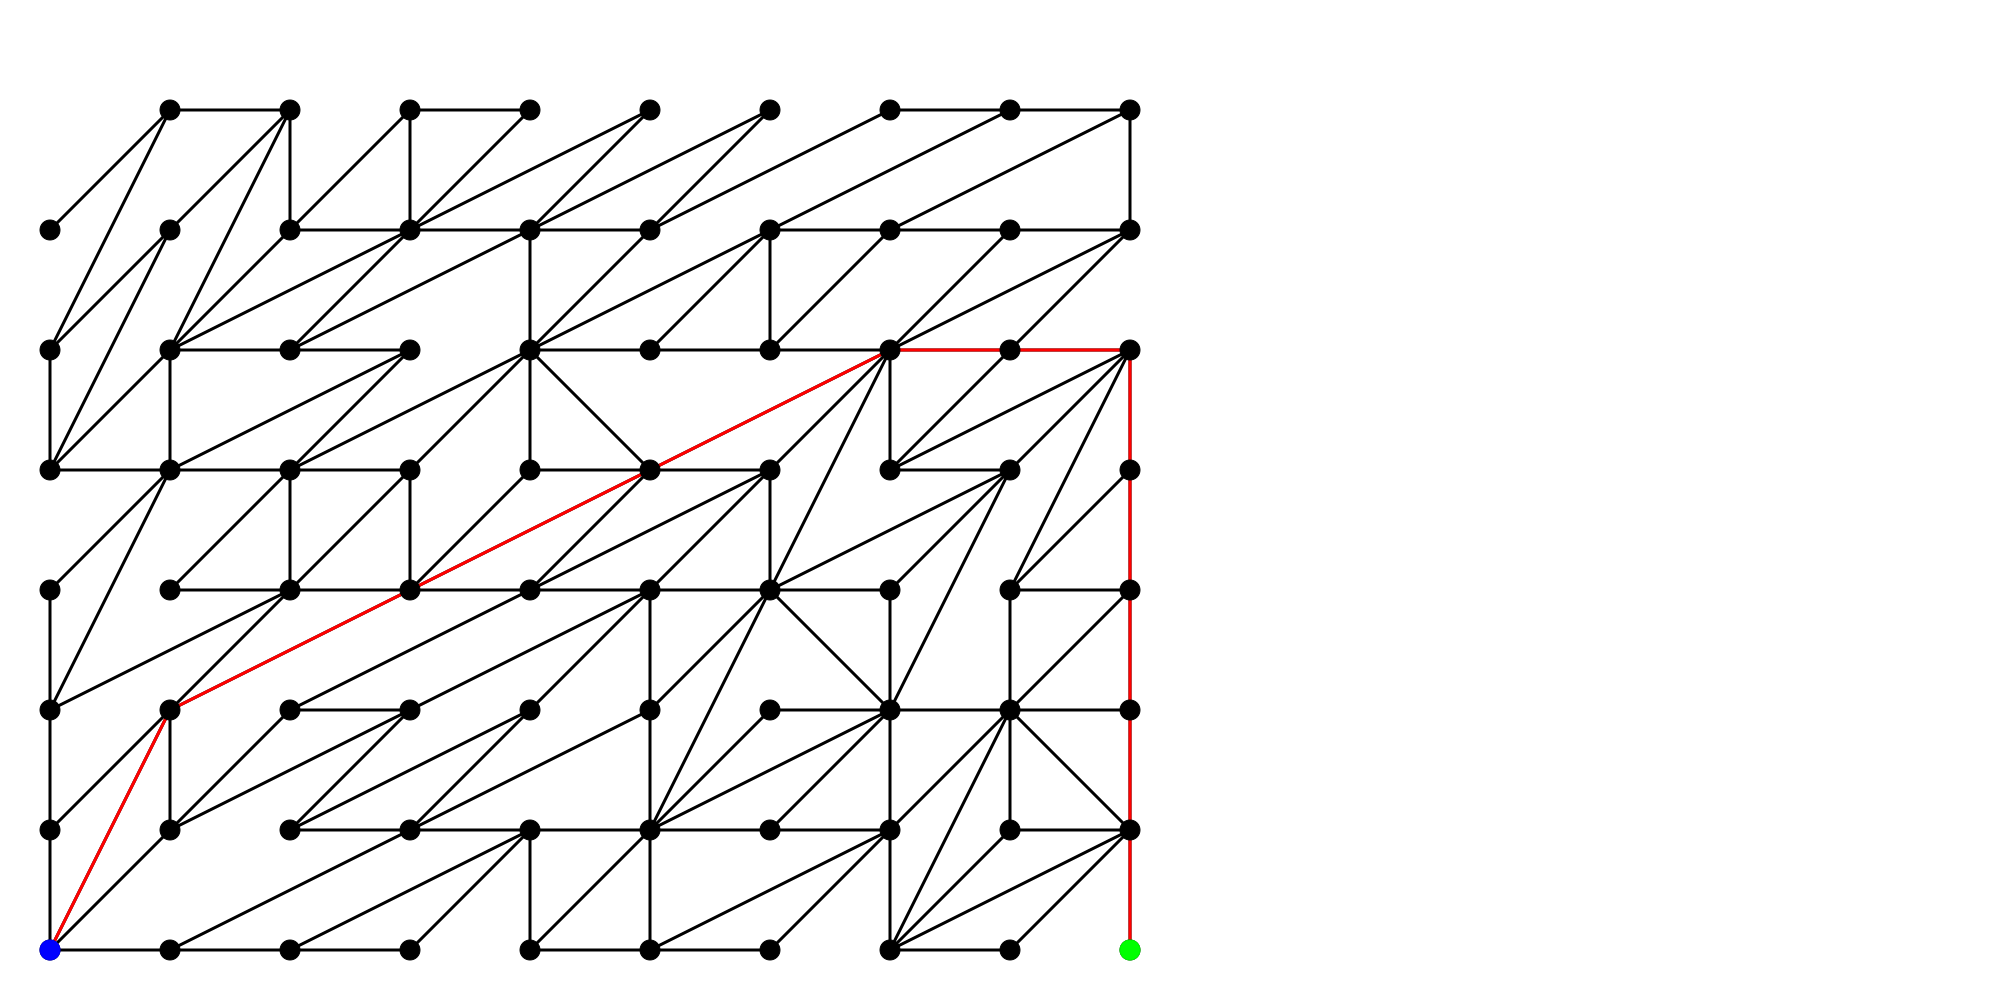
\includegraphics[scale=0.3]{abbiegen2leastTurns.png}
\end{center}
    \end{itemize}
\end{itemize}

\subsection{Beispiel 3 (BWINF)}
Textdatei: \texttt{abbiegen3.txt}

\begin{itemize}
  \item 110\%    
    \begin{itemize}
      \item Abbiegen: \textbf{4} (das beste Ergebnis)
      \item Länge des Pfades: \textbf{17,8863}
      \item Länge des Pfades prozentual: \textbf{104,462\%}
      \item Punkte: \textbf{(0, 0), (1, 1), (2, 1), (3, 1), (4, 1), (5, 1), (7, 2), 
      (9, 3), (10, 3), (11, 3), (12, 3), (13, 3), (14, 3), (14, 2), (14, 1), (14, 0)}
\begin{center}
\includegraphics[scale=0.26]{abbiegen3_10.png}
\end{center}
    \end{itemize}
  \item 115\%    
    \begin{itemize}
      \item Abbiegen: \textbf{4}
      \item Länge des Pfades: \textbf{17,8863}
      \item Länge des Pfades prozentual: \textbf{104,462\%}
      \item Punkte: \textbf{(0, 0), (1, 1), (2, 1), (3, 1), (4, 1), (5, 1), (7, 2), 
      (9, 3), (10, 3), (11, 3), (12, 3), (13, 3), (14, 3), (14, 2), (14, 1), (14, 0)}
\begin{center}
\includegraphics[scale=0.26]{abbiegen3_10.png}
\end{center}
    \end{itemize}
  \item 130\%    
    \begin{itemize}
      \item Abbiegen: \textbf{4}
      \item Länge des Pfades: \textbf{17,8863}
      \item Länge des Pfades prozentual: \textbf{104,462\%}
      \item Punkte: \textbf{(0, 0), (1, 1), (2, 1), (3, 1), (4, 1), (5, 1), (7, 2), 
      (9, 3), (10, 3), (11, 3), (12, 3), (13, 3), (14, 3), (14, 2), (14, 1), (14, 0)}
\begin{center}
\includegraphics[scale=0.26]{abbiegen3_10.png}
\end{center}
    \end{itemize}
  \item der kürzeste Pfad   
    \begin{itemize}
      \item Abbiegen: 7
      \item Länge des Pfades: 17,1224
\begin{center}
\includegraphics[scale=0.26]{abbiegen3shortest.png}
\end{center}
    \end{itemize}
\end{itemize}

\subsection{Beispiel 4}
Textdatei: \texttt{abbiegen4.txt}\\
Besonderheit: der Pfad mit der niedrigsten Anzahl von Abbiegungen ist gleich 0, der Pfad verläuft nur über den
Diagonalen

\begin{itemize}
  \item 110\%    
    \begin{itemize}
      \item Abbiegen: \textbf{0} (das beste Ergebnis)
      \item Länge des Pfades: \textbf{5,65685}
      \item Länge des Pfades prozentual: \textbf{100\%}
      \item Punkte: \textbf{(0, 0), (1, 1), (2, 2), (3, 3), (4, 4)}
\begin{center}
\includegraphics[scale=0.4]{abbiegen4_10_1.png}
\end{center}
  \end{itemize}
  \item 115\%: das Gleiche wie bei 110\%
  \item 130\%: das Gleiche wie bei 110\%
\end{itemize}

\subsection{Beispiel 5}
Textdatei: \texttt{abbiegen5.txt}\\
Besonderheit: sehr viele Abbiegungen im besten Pfad, das Ziel ist isoliert vom Rest des Graphen,
vom Punkt (4, 3) zum (3, 4) macht der Algorithmus einen Schritt zurück in Bezug auf die $x$-Achse (s. Lösungsidee)

\begin{itemize}
  \item 110\%    
    \begin{itemize}
      \item Abbiegen: \textbf{6} (das beste Ergebnis)
      \item Länge des Pfades: \textbf{9,65685}
      \item Länge des Pfades prozentual: \textbf{100\%}
      \item Punkte: \textbf{(0, 0), (1, 0), (2, 1), (1, 2), (2, 3), (3, 3), (4, 3), (3, 4), (4, 4)}
\begin{center}
\includegraphics[scale=0.4]{abbiegen5_10.png}
\end{center}
  \end{itemize}
  \item 115\%: das Gleiche wie bei 110\%
  \item 130\%: das Gleiche wie bei 110\%
\end{itemize}

\subsection{Beispiel 6}\label{zielindermitte}
Textdatei: \texttt{abbiegen6.txt}\\
Besonderheit: Da Ziel befindet sich nicht ,,am Ende'' der Matrix

\begin{itemize}
  \item 110\%    
    \begin{itemize}
      \item Abbiegen: \textbf{3} (das beste Ergebnis)
      \item Länge des Pfades: \textbf{7.23607}
      \item Länge des Pfades prozentual: \textbf{100\%}
      \item Punkte: \textbf{(1, 4), (2, 4), (4, 5), (5, 5), (6, 5), (7, 5), (7, 4)}
\begin{center}
\includegraphics[scale=0.3]{abbiegen6_10.png}
\end{center}
  \end{itemize}
  \item 115\%: das Gleiche wie bei 110\%
  \item 130\%: das Gleiche wie bei 110\%
\end{itemize}

\subsection{Beispiel 7}\label{nichtganzzahlige}
Textdatei: \texttt{abbiegen7.txt}\\
Besonderheit: nichtganzzahlige Koordinaten

\begin{itemize}
  \item 110\%    
    \begin{itemize}
      \item Abbiegen: \textbf{3} (das beste Ergebnis)
      \item Länge des Pfades: \textbf{13,4721}
      \item Länge des Pfades prozentual: \textbf{106,497\%}
      \item Punkte: \textbf{(0, 0), (1, 0), (2.5, 0.4), (4.3, 1.16), (5.2, 1.6), (7, 2), (9, 3), (11.5, 4.2), (11, 3), (12, 3), (13, 3), (14, 3), (14, 2), (14.4, 1.3), (14.5, 0.7)}
\begin{center}
\includegraphics[scale=0.27]{abbiegen7_10.png}
\end{center}
  \end{itemize}
  \item 115\%: das Gleiche wie bei 110\%
  \item 130\%: das Gleiche wie bei 110\%
  \item der kürzeste Pfad   
    \begin{itemize}
      \item Abbiegen: 3
      \item Länge des Pfades: 12,6503
\begin{center}
\includegraphics[scale=0.27]{abbiegen7shortest.png}
\end{center}
    \end{itemize}
\end{itemize}

\subsection{Beispiel 8}\label{kreuzen}
Textdatei: \texttt{abbiegen8.txt}\\
Besonderheit: Straßen kreuzen sich

\begin{itemize}
  \item 110\%    
    \begin{itemize}
      \item Abbiegen: \textbf{6}
      \item Länge des Pfades: \textbf{17,3006}
      \item Länge des Pfades prozentual: \textbf{101,04\%}
      \item Punkte: \textbf{(0, 0), (1, 1), (2, 1), (3, 1), (4, 1), (5, 1), (6, 2), (8, 3), (9, 1), (10, 1), (11, 1), (12, 1), (13, 1), (14, 1), (14, 0)}
\begin{center}
\includegraphics[scale=0.27]{abbiegen8_10.png}
\end{center}
  \end{itemize}
  \item 115\%    
    \begin{itemize}
      \item Abbiegen: \textbf{5} (das beste Ergebnis)
      \item Länge des Pfades: \textbf{19,1224}
      \item Länge des Pfades prozentual: \textbf{111,681\%}
      \item Punkte: \textbf{(0, 0), (1, 1), (2, 1), (3, 1), (4, 1), (5, 1), (7, 2), (9, 3), (11, 4), (11, 3), (12, 3), (13, 3), (14, 3), (14, 2), (14, 1), (14, 0)}
\begin{center}
\includegraphics[scale=0.27]{abbiegen8_15.png}
\end{center}
  \end{itemize}
  \item 130\%: das Gleiche wie bei 115\%
  \item der kürzeste Pfad   
    \begin{itemize}
      \item Abbiegen: 7
      \item Länge des Pfades: 17,1224
\begin{center}
\includegraphics[scale=0.27]{abbiegen8shortest.png}
\end{center}
    \end{itemize}
\end{itemize}

\subsection{Beispiel 2 (erweitert)}\label{genauigkeit}
Textdatei: \texttt{abbiegen2.txt}\\
Besonderheit: Anwendung der Möglichkeit der Wahl der Genauigkeit

\begin{itemize}
  \item 120\% (approximierte Suche)   
    \begin{itemize}
      \item Abbiegen: \textbf{4}
      \item Länge des Pfades: \textbf{13,0645}
      \item Länge des Pfades prozentual: \textbf{120\%} (eigentlich 120,008\%)
      \item Punkte: \textbf{(0, 0), (1, 0), (2, 0), (4, 1), (5, 1), (6, 1), (7, 1), (8, 2), (9, 3), (9, 2), (9, 1), (9, 0)}
  \begin{center}
  \includegraphics[scale=0.3]{abbiegen2_20ungenau.png}
  \end{center}
  \end{itemize}
  \item 120\% (genaue Suche)    
    \begin{itemize}
      \item Abbiegen: \textbf{5}
      \item Länge des Pfades: \textbf{12,7082}
      \item Länge des Pfades prozentual: \textbf{116,735\%}
      \item Punkte: \textbf{(0, 0), (1, 0), (3, 1), (5, 2), (5, 1), (7, 2), (8, 2), (9, 2), (9, 1), (9, 0)}
  \begin{center}
  \includegraphics[scale=0.3]{abbiegen2_20genau.png}
  \end{center}
  \end{itemize}
\end{itemize}

\newpage
\section{Quellcode}
Hier füge ich Implementierungen von zwei Methoden bei:
den Yen–Algotihmus und den Algorithmus, der die Kanten im Graphen $G'$ (Typ 2) erstellt.\\
Die Zeilenangaben beziehen sich auf die Zeilen im Pseudocode aus Wikipedia auf Seite \pageref{wikipedia.pseudo}.
\lstinputlisting[language=C++]{abbiegen.m}

\newpage
\section{Pseudocode aus Wikipedia}

Der mehrmals zitierte Pseudocode aus dem englischen Wikipedia-Artikel über den Yen-Algorithmus.\\
Quelle: \href{https://en.wikipedia.org/wiki/Yen%27s_algorithm#Pseudocode}
{\texttt{https://en.wikipedia.org/wiki/Yen\%27s\_algorithm\#Pseudocode}}, Zugang 15.03.2020\\

\begin{lstlisting}[language=C++]
function YenKSP(Graph, source, sink, K):
   // Determine the shortest path from the source to the sink.
   A[0] = Dijkstra(Graph, source, sink);
   // Initialize the set to store the potential kth shortest path.
   B = [];
   
   for k from 1 to K:
       // The spur node ranges from the first node to the 
       // next to last node in the previous k-shortest path.
       for i from 0 to size(A[k - 1]) - 2:
           
           // Spur node is retrieved from the previous k-shortest path, k - 1.
           spurNode = A[k-1].node(i);
           // The sequence of nodes from the source to the 
           // spur node of the previous k-shortest path.
           rootPath = A[k-1].nodes(0, i);
           
           for each path p in A:
               if rootPath == p.nodes(0, i):
                   // Remove the links that are part of the previous 
                   // shortest paths which share the same root path.
                   remove p.edge(i,i + 1) from Graph;
           
           for each node rootPathNode in rootPath:
               remove rootPathNode from Graph;
           
           // Calculate the spur path from the spur node to the sink.
           spurPath = Dijkstra(Graph, spurNode, sink);
           
           // Entire path is made up of the root path and spur path.
           totalPath = rootPath + spurPath;
           // Add the potential k-shortest path to the heap.
           if (totalPath not in B):
               B.append(totalPath);
           
           // Add back the edges and nodes that were removed
           // from the graph.
           restore edges to Graph;
           restore nodes in rootPath to Graph;
                   
       if B is empty:
           // This handles the case of there being no spur paths, 
           // or no spur paths left.
           // This could happen if the spur paths have already 
           // been exhausted (added to A), 
           // or there are no spur paths at all - such as when both 
           // the source and sink vertices 
           // lie along a "dead end".
           break;
       // Sort the potential k-shortest paths by cost.
       B.sort();
       // Add the lowest cost path becomes the k-shortest path.
       A[k] = B[0];
       // In fact we should rather use shift since we are 
       // removing the first element
       B.pop();
   
   return A
\end{lstlisting}\label{wikipedia.pseudo}

\newpage
\section{GUI}

\begin{figure}[h]
\centering
\includegraphics[scale=1.6]{gui-instructions.png}
\end{figure}

\begin{enumerate}
  \item Man wählt eine Datei aus, in der sich ein Beispiel befindet. Standardmäßig wird
  der Ordner \texttt{./input} geöffnet. (s. \texttt{ReadMe})
  \item Man gibt die maximale prozentuale Verlängerung ein.
  Dann klickt man auf \textit{OK} oder drückt
man \texttt{RETURN} auf der Tastatur.\\ \textbf{Wichtig:} Man gibt das Prozentzeichen nicht ein.
  \item Man wählt, ob man eine approximierte Suche durchführen möchte.
  \item Mit allen Angaben von 1 bis 3 klickt man auf \textit{Start}, indem man das Programm laufen lässt.
  \item Hier wird die Ausgabe angezeigt. Es wird der gefundene Pfad, die Punkte in diesem Pfad sowie
  der kürzeste Pfad von allen und der Pfad, bei dem man am wenigstens abbiegt, angezeigt.
  \item \textit{Default save} ordnet automatisch den SVG--Grafiken ihre Namen zu.\\
  Eine Eingabe von einer maximalen Verlängerung von 10 wird als \texttt{abbiegen\_10.svg} formattiert.\\
  Bei der gewählten Option der approximierten Suche wird noch der folgende Teil hinzugefügt: \texttt{\_approx}.
  \item Hier kann man die generierte SVG--Grafik mit dem gefundenen Pfad speichern. Standardmäßig wird der Ordner
\texttt{./output} geöffnet und die Datei mit dem angezeigten Namen gespeichert.
  \item Hier kann man die generierte SVG--Grafik mit dem kürzesten Pfad speichern. Standardmäßig wird der Ordner
\texttt{./output} geöffnet  und die Datei mit dem angezeigten Namen gespeichert.
  \item Hier kann man die generierte SVG--Grafik mit dem Pfad, bei dem man am wenigsten abbiegen muss, speichern. Standardmäßig wird der Ordner
\texttt{./output} geöffnet und die Datei mit dem angezeigten Namen gespeichert.
  \item Hier kann man alle SVG--Grafiken gleichzeitig mit einem Klick speichern. Standardmäßig werden sie im Ordner
\texttt{./output} mit den angezeigten Namen gespeichert).
\end{enumerate}

\end{document}